
\documentclass[tikz,convert={convertexe={magick.exe}}]{standalone}

\begin{document}
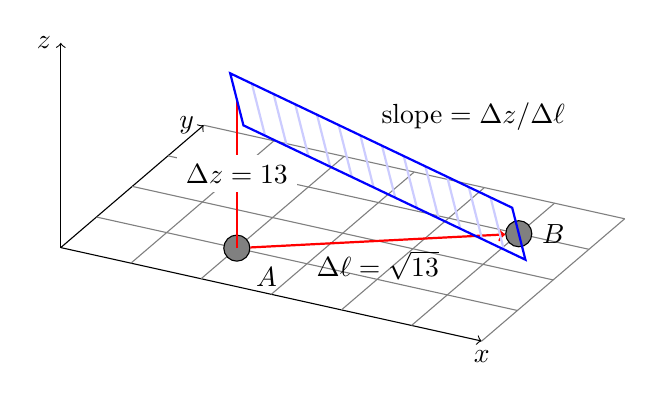
\begin{tikzpicture}

\draw[->] (0.000,0.000)--(5.346,-1.187) node[below] {$x$};
\draw[->] (0.000,0.000)--(1.816,1.554) node[left] {$y$};
\draw[->] (0.000,0.000)--(0.000,2.6) node[left] {$z$};
\draw[gray] (0.891,-0.198)--(2.707,1.356);
\draw[gray] (1.782,-0.396)--(3.598,1.158);
\draw[gray] (2.673,-0.594)--(4.489,0.960);
\draw[gray] (3.564,-0.792)--(5.380,0.762);
\draw[gray] (4.455,-0.989)--(6.271,0.564);
\draw[gray] (5.346,-1.187)--(7.162,0.366);
\draw[gray] (0.454,0.388)--(5.800,-0.799);
\draw[gray] (0.908,0.777)--(6.254,-0.411);
\draw[gray] (1.362,1.165)--(6.708,-0.022);
\draw[gray] (1.816,1.554)--(7.162,0.366);


\node[circle, draw, fill=gray, label=below right:{$A$}] (A) at (2.236,-0.007) {};
\draw[red,thick] (2.236,-0.007) --(2.236,1.883) node[midway, black, fill=white] {$\Delta z = 13$};
\node[circle, draw, fill=gray, label=right:{$B$}] (B) at (5.817,0.176) {};

\draw[red,thick,->] (A) -- (B) node[midway, black, below] {$\Delta \ell = \sqrt{13}$};

\draw[blue!20,thick] (2.427,2.081)--(2.595,1.421);
\draw[blue!20,thick] (2.703,1.950)--(2.871,1.290);
\draw[blue!20,thick] (2.978,1.819)--(3.146,1.159);
\draw[blue!20,thick] (3.254,1.688)--(3.422,1.027);
\draw[blue!20,thick] (3.529,1.556)--(3.697,0.896);
\draw[blue!20,thick] (3.805,1.425)--(3.973,0.765);
\draw[blue!20,thick] (4.080,1.294)--(4.248,0.633);
\draw[blue!20,thick] (4.356,1.162)--(4.524,0.502);
\draw[blue!20,thick] (4.631,1.031)--(4.799,0.371);
\draw[blue!20,thick] (4.907,0.900)--(5.075,0.239);
\draw[blue!20,thick] (5.182,0.768)--(5.350,0.108);
\draw[blue!20,thick] (5.458,0.637)--(5.626,-0.023);
\draw[blue,thick] (2.152,2.213)--(5.733,0.506) node[midway, black, above right] {$\mathrm{slope} = \Delta z / \Delta \ell$}--(5.901,-0.154)--(2.320,1.552)--cycle;

\end{tikzpicture}
\end{document}